\documentclass[a4paper, 12pt]{article}

\usepackage[ a4paper,
 total={170mm,257mm},
 left=20mm,
 top=20mm,]{geometry}

\usepackage{cmap}
\usepackage[T2A]{fontenc}
\usepackage[utf8]{inputenc}
\usepackage[english, russian]{babel}

%Графика
\usepackage{graphicx}
\usepackage{float}%"Плавающие" картинки
\usepackage{wrapfig}%Обтекание фигур (таблиц, картинок и прочего)
\graphicspath{{./images/}}

% Математика
\usepackage{amsmath,amsfonts,amssymb,amsthm,mathtools} 

%Title Page
\title{ЛАБОРАТОРНАЯ РАБОТА № 1 \\
Моделирование механических систем
}
\author{Вариант 11 \\ Машуров Владимир БПМ-19-3}

\setcounter{page}{0}

\begin{document}
\maketitle
\thispagestyle{empty}
\newpage
\tableofcontents

\section{Моделирование механической системы масса-пружина}

Дана система:

\begin{equation}
M\dot{x} + B\dot{x} + kx = f(t)
\label{СистемаСБлокомНаПружинеИДемпфером}
\end{equation}

Где $f(t)$ - входное воздействие, $x(t)$ - выходное воздействие.
 
\textbf{Задание 1.1 } \\
Применив преобразование Лапласа (с нулевыми начальными условиями) найдите передаточную функцию модели: $ G(s) = \frac{X(s)}{F(s)} $ 

Найдём соотношение из которого получим G(t):


$$M\dot{x}(t) + B\dot{x}(t) + kx(t) = f(t) \; \; \; \frac{d}{dt} = \lambda $$

$$ M\lambda^2x(t) + B\lambda x(t) + kx(t) = f(t) $$

$$ (M\lambda^2 + B\lambda + k)x(t) = f(t) $$

$$ \frac{x(t)}{f(t)} = \frac{1}{M\lambda^2 + B\lambda + k} $$

Отсюда

$$ G(s) = \frac{X(s)}{F(s)} = \mathcal{L} \bigg( \frac{x(t)}{f(t)} \bigg) = \frac{\mathcal{L}(\tilde{x}(t))}{\mathcal{L}(\tilde{f}(t))} = $$
$$ = \frac{\mathcal{L}(1)}{\mathcal{L}(M\lambda^2 + B\lambda + k)} =  \frac{1}{s} \cdot \frac{s}{M\lambda^2 + B\lambda + k} = \frac{1}{M\lambda^2 + B\lambda + k} $$

\textbf{Задание 1.2 } \\
Перепишите уравнение \ref{СистемаСБлокомНаПружинеИДемпфером} в форму вход-состояние-выход.

$$M\ddot{x}(t) + B\dot{x}(t) + kx(t) = f(t) $$ 

Разделим всё на $M$ и заменим переменные следующим образом, для удобства: $f = U$ и $x = y$. Получим 

$$ \ddot{y} + \frac{B}{M}\dot{y} + \frac{k}{M}y = \frac{1}{M}U $$

Составим систему:

$$ \begin{cases}
x_1 = y \\
x_2 = \dot{y} + \frac{B}{M} y
\end{cases} $$

Продифференцируем оба равенства по $t$

$$ \begin{cases}
\dot x_1 = \dot y = x_2 - \frac{B}{M} y \\
\dot x_2 = \ddot y +\frac{B}{M} \dot y = \frac{1}{M} U - \frac{k}{M} y = \frac{1}{M} U - \frac{k}{M} x_1
\end{cases} $$

Мы пришли к форме вход-состояние-выход. Обратим замену переменных:

$$ \begin{cases}
\dot \pi_1 = \pi_2 - \frac{B}{M} x \\
\dot \pi_2 = \frac{1}{M} f - \frac{k}{M} \pi_1
\end{cases} $$

\textbf{Задание 1.3 } \\
Составьте структурную схему моделирования, опираясь на уравнение \ref{СистемаСБлокомНаПружинеИДемпфером} и результат, полученный в Задании 2.

$$M\ddot{x}(t) + B\dot{x}(t) + kx(t) = f(t) \; \; \; |:M $$

$$\ddot{x}(t) + \frac{B}{M}\dot{x}(t) + \frac{k}{M}x(t) = \frac{1}{M} f(t) $$

$$ \ddot{x}(t) = \frac{1}{M} f(t) - \frac{k}{M}x(t) - \frac{B}{M}\dot{x}(t) \; \; \; |\frac{d}{dt} = \lambda$$

$$ \lambda^2 x(t) = \frac{1}{M} f(t) - \frac{k}{M}x(t) - \frac{B}{M} \lambda x(t) \; \; \; |:\lambda^2$$

$$ x(t) = \frac{1}{\lambda^2} \Big( \frac{1}{M} f(t) - \frac{k}{M}x(t) \Big) -\frac{1}{\lambda} \Big( \frac{B}{M} x(t) \Big) \; \; \; |:\lambda^2$$


Из полученного выражения можно построить структурную схему, изображенную на рисунке \ref{p:Схема1}.

\begin{figure}[h!]
	\centering
	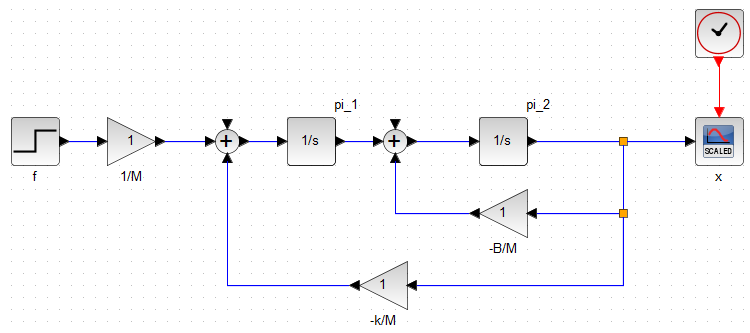
\includegraphics[scale=0.6]{scheme1}
	\caption{Структурная схема моделирования механической системы масса-пружина }
	\label{p:Схема1}
\end{figure}

\newpage
\section{Исследование модели вход-состояние-выход}

\end{document}